\documentclass[aps,twocolumn,secnumarabic,balancelastpage,amsmath,amssymb,nofootinbib]{revtex4}
%\documentclass[aps,twocolumn,secnumarabic,balancelastpage,amsmath,amssymb,nofootinbib]{revtex4-1}

\usepackage{chapterbib,color,graphics,longtable,epsf,bm,thumbpdf}
\usepackage[pdftex]{graphicx}
%\usepackage{asymptote}     
\usepackage[colorlinks=true]{hyperref}  


\begin{document}
\title{Proposal for Counter-Propagating Beam Instability and Transverse-Pattern Formation in Warm Rubidium Vapor}
\author{G. Resta}
\email{gresta@mit.edu}
\author{Y. Yu}
\email{yuyichao@mit.edu}
%\homepage{http://web.mit.edu/8.13/}
\date{\today}
\affiliation{Junior Lab B02 - MIT Department of Physics}

\begin{abstract}
We propose and describe an experimental setup to investigate spacial polarization instabilities and transverse-pattern formation resulting from the counter-propagation of two laser beams in warm rubidium vapor. In addition to reproducing the effect, our intent is to quantify variations in the pattern as a function of frequency and beam profile inhomogeneity resulting from either altering the distance traveled or amount of power in one of the two beams. 
\end{abstract}

\maketitle
\subsection*{Introduction}
The study of pattern formations in physical systems has long been the subject of fascination. 
%Pattern formation concerns itself with the presence of visible order throughout the evolution of a system. 
In the field of non-linear optics, recent observations of ``Flower-like Patterns'' generated by heated rubidium vapor have identified a series of formations unique from those observed in other passive nonlinear medium\cite{grynberg93}. Even more recently, this effect has acquired a fair amount of interest for potential applications in an all-optical switch, demonstrating sensitivity levels far exceeding those currently observed by similar Electromagnetically-Induced Transparency (EIT) solutions\cite{duke01}. We hope that by reproducing the effect, using components from the Doppler-Free apparatus, we will not only study a unique non-linear optical phenomena, but also open the possibility for a future group to study an all-optical switch.

\subsection*{Nature of Polarization Instability and Pattern Formation}
When two laser beams of an identical frequency counter-propagate upon each other they generate a series of standing waves. If these standing waves are located within a non-linear optical medium, areas of the medium where the waves constructively interfere behave differently from areas of the medium where the waves destructively interfere. In the case of polarization instabilities, atoms within regions of constructive interference have more aligned spins then atoms in regions of destructive interference. This periodic variation tends to amplify weak occurrences of light with specific polarization modes. Since these polarization modes increase in amplitude drastically, the phenomena is referred to as counter-propagating beam instability as the amplitudes of certain modes within the system are unstable.

\subsection*{Optical Layout}
Figure~\ref{fig:layout} illustrates the proposed optical layout for our experiment. The beam-line begins with a laser having a central wave-length of around 780nm corresponding to the rubidium $5S_{1/2}-5P_{3/2}$ transition and a frequency de-tuning capability on the order of 10GHz. Light from the laser is fed through a Faraday Isolator with the aim of preventing any returning light from destabilizing or damaging the laser. Following the isolator, the beam is channeled into a fiber optic coupler with the aid of an appropriate lens. The fiber optic coupler acts to modify the laser beam into a circular Gaussian profile. While deviations from a circularly profile would diminish the generation of instability, if the laser has a sufficiently circular aperture this step may not be strictly necessary. Following the fiber optic coupler, the beam is first collimated by a lens and then sent through a half-wave plate which allows for the polarization of the light to be rotated into the appropriate plane such that it is not reflected by the polarization beam splitter positioned after the rubidium vapor cell. A polarization filter (depicted) may be necessary after the half-wave plate if we find that the laser is not coherently polarized along a single axis after traveling through the fiber optic coupler. 

\begin{figure}[h!]
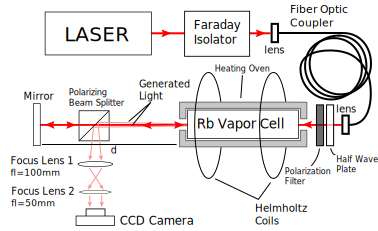
\includegraphics[width=0.9\linewidth]{drawing.png}
\caption{\label{fig:layout} Schematic depiction of proposed optical beam-line. Note that the setup would allow for the possible to split the laser beam shortly after the \textit{Faraday Isolator} to allow for an additional optical beam-line setup in tandem (not shown).}
\end{figure}

Once the polarization of the beam is adjusted, the light is sent through a rubidium cell that is heated by an oven which minimizes any stray magnetic fields and maintains the windows of the cell at a higher temperature than the interior. Openings on either side of the oven should allow for a 5mrad beam of light originating from the other side of the cell to pass unobstructed. The length of the rubidium cell should ideally be as long as possible (the amplitude of the electric field resulting from the instability scales with the product of the atomic density and the length of the cell). The laser light should likewise incident the windows of the cells at an angle of approximately 10 degrees to insure that any light reflected from the window surfaces does not interfere with the rest of the system. 

The function of the oven is to increase the atomic density of rubidium within the cell. While the ideal temperature varies from cell to cell, it is expected that maintaining the rubidium vapor at a temperature from around 68 to 90 degrees Celsius should be sufficient for obtaining an atomic density on the order of $10^{12}$ atoms/cm$^3$ and thereby observing the effect.

After traveling through the vapor cell, the laser beam is sent through a polarizing beam-splitter. While within discussed studies this splitter consisted of a Glan prism\cite{grynberg93}, in principle any beam-splitter which leaves incident light polarized in a particular direction unaffected and reflects incident light polarized orthogonally to that particular direction should be sufficient.

Finally the incident light from the laser is reflected by a mirror located at a variable distance $d$ from the end of the cell in such a way as to be propagated back through the polarizing beam-splitter and through the cell superimposed on the direct beam. The setup should allow for the mirror to be varied from between 10 to 30 cm from the end of the vapor cell. It appears that the tolerance on the alignment between these two beams is comparable to that of a Fabry-Perot cavity. Once this alignment has been established and the two counter-propagating beams succeed in developing a series of standing waves within the rubidium vapor, light generated from the resulting instability should be emitted with a divergence of 5mrad from the vapor cell onto the polarizing beam-splitter. Since the generated light should have a polarization orthogonal to the incident beam, it should be reflected from the splitter onto a series of lens, focusing the signal onto a CCD camera.   


\subsection*{Heater Design}

The design of the heater is in many ways the most critical and untested part of our experiment. We have resolved against solutions that use air as a conductive medium on the note that such a technique may interfere with the incident light. Instead we have decided that designs using a heating element in contact with a machined block of metal surrounding the cell would be most suitable. Figure~\ref{fig:heater} illustrates the heater design currently under consideration. It consists primarily of four half-cylindrical heaters surrounding two machined aluminum blocks in which the cell rests. The heating coils are looped around their encasing in such a way as to minimize magnetic fields. Likewise, by locating the windows of the cell toward the center of the heating coils and having the center of the cell exposed to the surrounding air, the design insures that the center of the cell is maintained at a lower temperature than the windows, preventing condensation. To generate heat, the coils should be connected to a variable DC power supply as oppose to an AC power supply to suppress the generation of any type of oscillating magnetic fields. Likewise, a temperature controller found near the M\"ossbauer equipment could be used to regulate the applied current provided that the controller is capable of managing DC current. An estimate for the amount of current required to heat the cell is difficult given the untested nature of the coils. However, a similar coil design mentioned in a study required 20.5 V at 0.76 A\cite{sclark04}. It is expected that our design may requires slightly more due to the fact that it is much larger than the design in the study. 

\begin{figure}[h!]
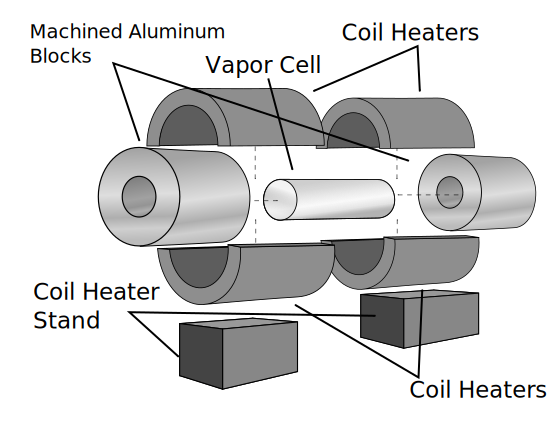
\includegraphics[width=0.8\linewidth]{heater.png}
\caption{\label{fig:heater} Schematic conceptual rendering of a heater using a series of large half-cylindrical heating coils. The usage of machined aluminum blocks is expected to facilitate an even distribution of heat to the vapor cell. }
\end{figure}

There is a certain concern that the snaking of the coils is insufficient to suppress the generation of magnetic fields. It has been suggested that the design could be improved by using thermoelectric heaters as opposed to coils. While this would drastically reduce any magnetic fields, it remains unclear whether such heaters can maintain the desired temperatures.

Regardless, due to the essential role of the heater in our experiment, we suggest that prior to our alloted experiment time we conduct a simple test, without the rubidium cell, to insure that the designed heater is able to reach the desired temperatures in a reliable fashion without generating excessive magnetic fields.

\subsection*{Helmholtz Coil Specifications}

A series of Helmholtz coils may need to be designed to reduce any type of systematic magnetic fields generated by the heater coils. To determine whether Helmholtz coils are necessary, we would like to measure the amount of magnetic field generated by the heater design in a test prior to our experiment time. A series of coils used in a similar study required two, 30 turn loops of copper wire with a radius of 12 cm separated by a distance of 12 cm with around 1A of applied current\cite{sclark04}. However, if we determine that our heater generates complicated magnetic fields that would inadequately be minimized by a set of Helmholtz coils, then, as a last resort, we could simply turn off the heater prior to making any fine measurements. 

\subsection*{Expected Analysis}
Once the beam-line is assembled and the expected signal appears on the CCD camera, we would proceed to analyze how the signal changes with variations in the frequency detuning of the laser, the mirror to cell distance $d$ and small perturbations in the alignment between the two beams. Is is expected that under variations in $d$, the number of petals composing the instability pattern undergoes abrupt changes\cite{grynberg93}. A formal description of this behavior can be understood in terms of Laguerre-Gauss modes. Likewise, we could insert an additional polarizing filter after the beam splitter to study variations in the pattern resulting from modifying the difference in power between the two beams.    

\subsection*{Conclusion}
We have presented technical details on implementing an experiment which demonstrates transverse pattern formation resulting from polarization instabilities in the counter-propagation of two laser beams in heated rubidium vapor.

\bibliography{paper}

\begin{acknowledgments} 
The authors would like to thank the technical staff for discussion.
\end{acknowledgments}

\clearpage
\appendix


\end{document}
